% !TEX root = ../Thesis.tex
\chapter{Experiments}\label{Experiments}
This chapter elaborates on how the different encodings perform and how the different Sudoku Variants compare.
The program to encode the various  puzzle instances is written in Java. We also use Java to call the different solvers (introduced in \ref{MiniSatAndSat4j}) and to log the resulting data. All experiments are run on a personal computer using Windows 10. The PC has an AMD Ryzen 7 5800X 8-Core Processor (3.80 GHz) and 32 GB of RAM (from which the Java Virtual Machine (JVM) is allowed to use 28GB).\\

The configurations we test for each puzzle instance differ by: 
\begin{itemize}
    \item The used Solver: Sat4j or MiniSat
    \item The used PBC-Encoding: Binary Decision Diagrams or Adder Networks
    \item The used optimization level: what is encoded as PBC (only for Killer Sudoku)
\end{itemize}

Conducting runtime experiments on a personal computer using Java comes with the caveat that the reported times all include some noise because their executions may be affected by other processes running in the background or by JVM events like garbage collections. To mediate that, we run 60 instances for every experiment configuration and report the average runtime and corresponding standard deviations.\\


Early testing showed that the solving times depend heavily on the order in which clauses and literals are given to the solvers. This is critical because we store clauses in sets and treat them as sets themselves. So the order of clauses (and literals) is not strictly defined and can vary from run to run. To still obtain comparable results, we order the clauses by length and the literals by the absolute values that encode them. We arbitrarily decided to pass the clauses containing the most literals first and to sort the literals within a clause by increasing absolute values. This way, the solvers get the same encoding as input if a problem is encoded and solved multiple times. However, eliminating this additional noise comes at the cost of having to sort all the clauses after they are created.
\newpage
Because we use a relatively small test set of different puzzle instances, it is important to note that assumptions made based on insights from the conducted experiments may not be applied to a general case. The reason for the limited size of the test set is that in the case of puzzles from CTCGH, they are very exotic and often unique. For Killer Sudokus Puzzles, many instances can be found, but writing the puzzle down into a format that the program can work on is very time-consuming as it has to be done manually.

\section{Adder Networks vs. Binary Decision Diagrams}
To analyze the Encoding of PBCs, we conducted further experiments using Killer Sudoku instances from the books ``The Times Ultimate Killer Su Doku Book 14"\cite{TheTimesUltimateKillerSuDokuBook14} and ``The Times Killer Su Doku (Book 18)''\cite{TheTimesKillerSuDokuBook18} both of which are the latest collections of Killer Sudoku Puzzles arranged by ``The Times''. In these books, puzzles are further categorized into categories of hardness, which reach from the easiest, ``Moderate'', to ``Extra Deadly'', the hardest. With ten instances from each of the categories, ``Moderate" and  ``Extra Deadly'', we can compare how Binary Decision Diagrams and Adder Networks perform when encoding PBCs.\\
\\
As Plot \ref{killerBDDencode} shows, there is a strong correlation between the number of clauses and the time needed to encode if BDDs are used. In the case of Adder Networks (Plot \ref{killerANencode}), it is harder to make such a statement, as some instances with few clauses require more time to encode compared to instances with fewer clauses. Furthermore, in this case, the variance in clauses needed by the instances is relatively low. So to reliably analyze the relation, additional samples with higher clause numbers would be necessary. \\
\\
Looking at the ratio of solving time per clause (shown in Plots \ref{killerBDDsolve} and \ref{killerANsolve}), it seems that in both cases, the variance in solving time between the different instances seems to increase the more clauses are needed to encode them.\\
\\
Finally, when comparing the solving times (Plot \ref{killerCompareSolve}), one can see that neither encoding with BDDs nor encoding with Adder Networks gives a clear advantage, as it depends on the puzzle instance, which method leads to a faster solving process. However, using Adder Networks has the advantage of being much faster in the encoding part itself, which can be seen in Plot \ref{killerCompareEncode}.\\
\\
Additionally, as one can see in the corresponding plots of this section, there also seems to be a clear trend that the Sudoku instances of the harder ``Extra Deadly'' category demand more clauses to encode them. However, this does not necessarily mean that they take longer to encode, or at least not if Adder Networks are used (see \ref{killerANencode}). If it comes to the time needed by the solver, it may seem intuitive that puzzles that are hard to solve for humans also take longer to be solved by a SAT-solver. Surprisingly this assumption which is by no means trivially given seems to be correct, as Plot \ref{killerCompareSolve} shows. 

\section{Optimization of Killer Sudoku Encoding}
Using the same Killer Sudoku Instances as explained in the previous section and Adder Networks to encode PBCs, we can compare the encoding and solving times of the two optimization ideas introduced in \ref{encoding:killer} to the standard approach of using PBCs. Plots \ref{opt_encode_2_1} and \ref{opt_solve_2_1} show that only generating the PBC for possible value combinations given the cages size and target sum leads to a measurable but neglectable performance gain. However, encoding Killer Sudokus completely without using PBCs can result in large savings, especially in solving time (see \ref{opt_encode_3_1} and \ref{opt_solve_3_1}).

\section{CTCGH Sudoku Variants compared using Sat4j and MiniSat}
Table \ref{Experimnet:CTCGH} shows the  outcome of encoding and solving thirteen different Sudoku instances with Sat4j and MiniSat. For puzzles where PBCs were needed, Adder Networks were used to encode them. The shown puzzle instances are from CTCGH and combine different variants and rules, except for ``Sudoku Man Of Mystery'' and ``The Road To Genius'', where only the normal Sudoku rules apply. An overview of which rules are present in each instance is given in Table \ref{tab:InstanceRule}.\\

Studying Table \ref{Experimnet:CTCGH}, one can see that in most cases the solving times using MiniSat are significantly higher than the ones of Sat4j. This may have to do with the fact that the Sat4j library and its functions can be accessed directly by the Java program, whereas the MiniSat-Solver is called as an external executable. For all further experiments, we are only using Sat4j (which internally also contains a version of MiniSat). There are two exceptions to Sat4j always being faster. ``The Original Sandwich'' and ``Nurikabe Sudoku'' seem to perform much better with MiniSat, which we have no direct explanation for. As shown in Table \ref{Experimnet:CTCGH}, those are the puzzle instances that demand the highest number of clauses and variables, which also means they potentially require more memory (we measured usage of up to 27 GB in the case of ``Nurikabe Sudoku''). Therefore, we think the external MiniSat executable might gain an advantage because of more efficient memory management than the Java-based solver. However, we do not have enough data to prove this claim, so MiniSat may prevail for other puzzle instances we did not test. Because the solving times for ``Nurikabe Sudoku'' using Sat4j are significantly higher, only ten runs were conducted instead of 60 like for the other puzzle instances.\\

When analyzing the constraints of ``Nurikabe Sudoku'', we found that the high number of clauses needed is mainly caused by the constraints ensuring that the ocean and every island is continuous. The Formulae NK-\ref{NK-xii}, NK-\ref{NK-xiii}, NK-\ref{NK-xiv}, NK-\ref{NK-xxi}, NK-\ref{NK-xxii} and NK-\ref{NK-xxiii} produce more than 12 million clauses alone, which is almost ten times the number all other instances require combined.\\

Comparing encoding to solving times (using Sat4j), it turns out that for instances without PBCs, the encoding times are all higher than the solving times, which does not hold if PBCs are involved, where it differs from instance to instance which part takes longer.






\clearpage
\FloatBarrier
{
\renewcommand{\figurename}{Plot}

\begin{figure}
    \centering
    \vspace{8.7mm}
    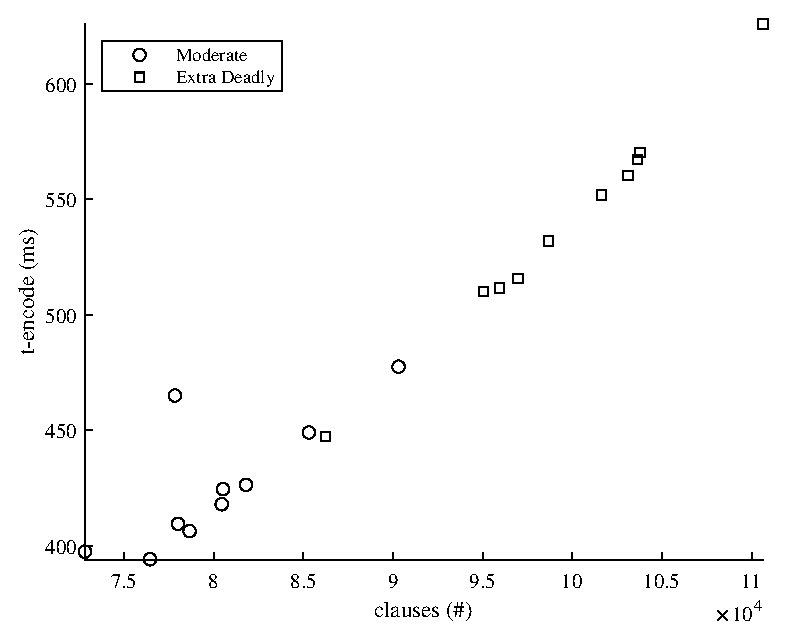
\includegraphics[height = 90mm]{Figures/killer_BDD_encode.eps}
    \caption{Encoding time per clause, using Binary Decision Diagrams}
    \label{killerBDDencode}
\end{figure}

\begin{figure}
    \centering
    \vspace{11mm}
    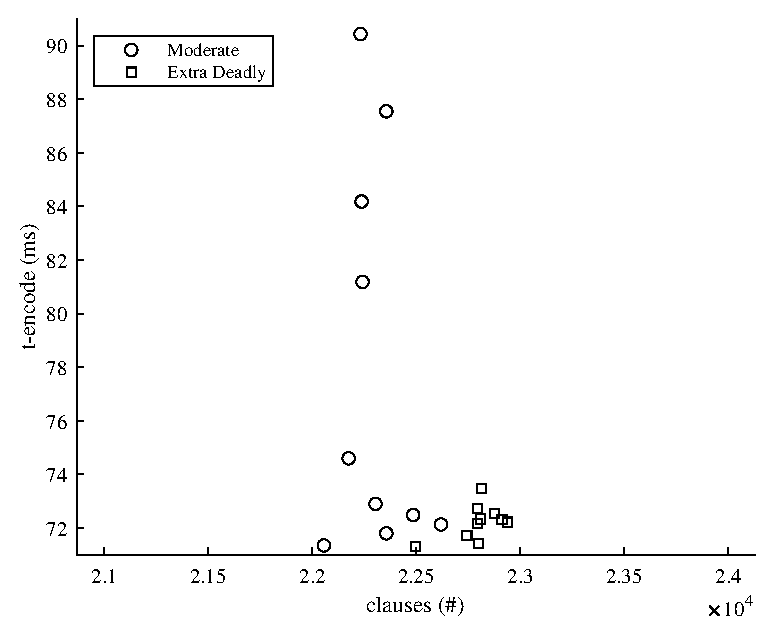
\includegraphics[height = 90mm]{Figures/killer_AN_encode.eps}
    \caption{Average encoding time per clause, using Adder Networks}
    \label{killerANencode}
\end{figure}

\begin{figure}
    \centering
    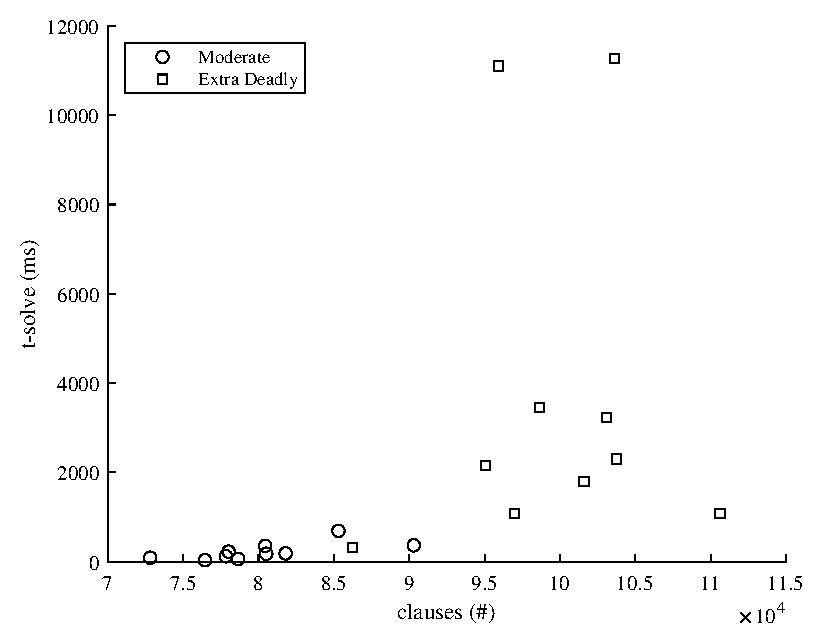
\includegraphics[height = 90mm]{Figures/killer_BDD_solve.eps}
    \caption{Average solving time per clause, using Binary Decision Diagrams}
    \label{killerBDDsolve}
\end{figure}

\begin{figure}
    \centering
    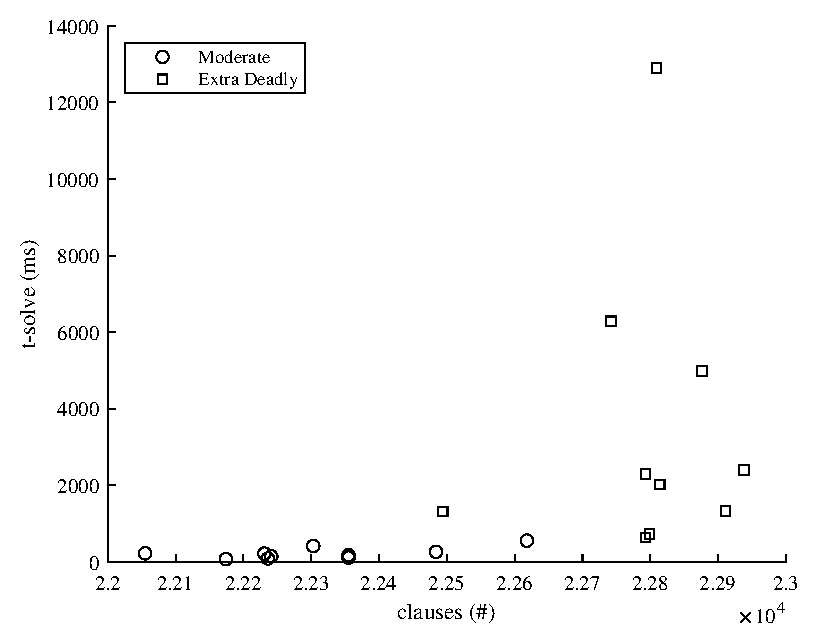
\includegraphics[height = 90mm]{Figures/killer_AN_solve.eps}
    \caption{Average solving time per clause, using Adder Networks}
    \label{killerANsolve}
\end{figure}

\begin{figure}
    \centering
    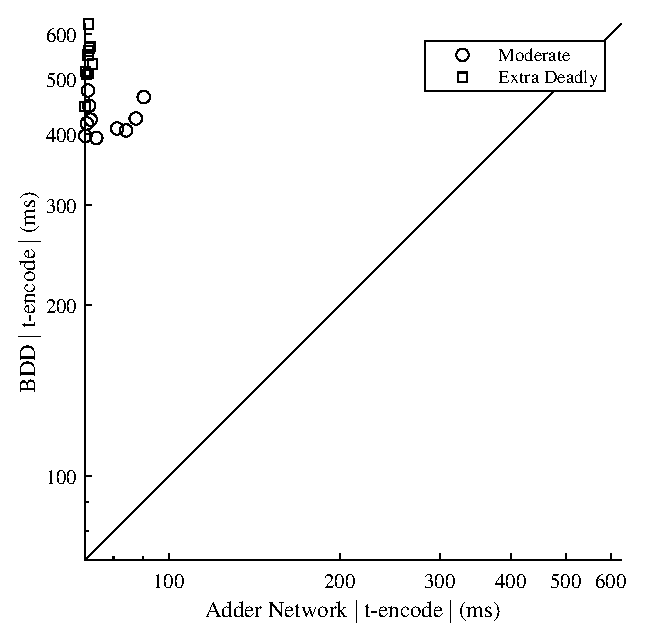
\includegraphics[height = 90mm]{Figures/killer_encode_compare.eps}
    \captionsetup{justification=centering,margin=0cm}
    \caption{Average encoding time comparison, Binary Decision Diagrams vs.\\Adder Networks}
    \label{killerCompareEncode}
\end{figure}

\begin{figure}
    \centering
    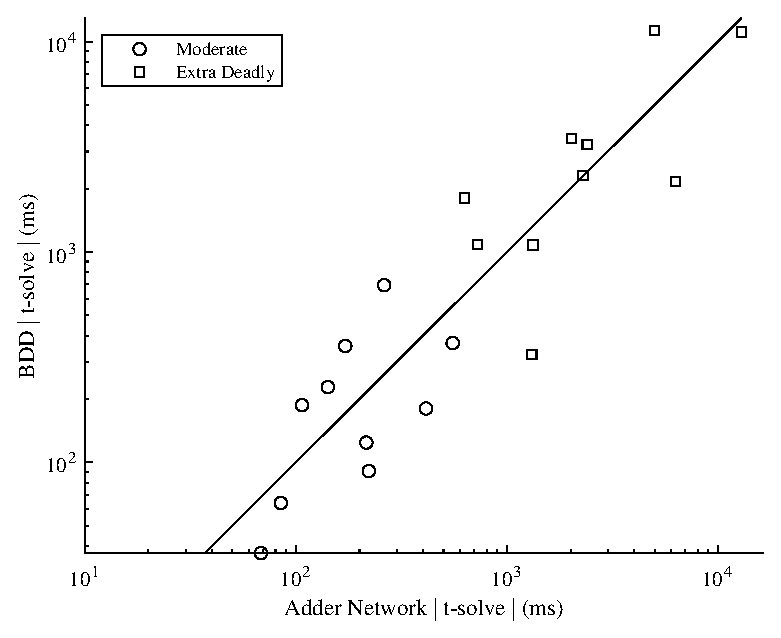
\includegraphics[height = 90mm]{Figures/killer_solve_compare.eps}
    \captionsetup{justification=centering,margin=0cm}
    \caption{Average solving time comparison, Binary Decision Diagrams vs.\\Adder Networks}
    \label{killerCompareSolve}
\end{figure}
}

{
\renewcommand{\figurename}{Plot}
\begin{figure}
    \centering
    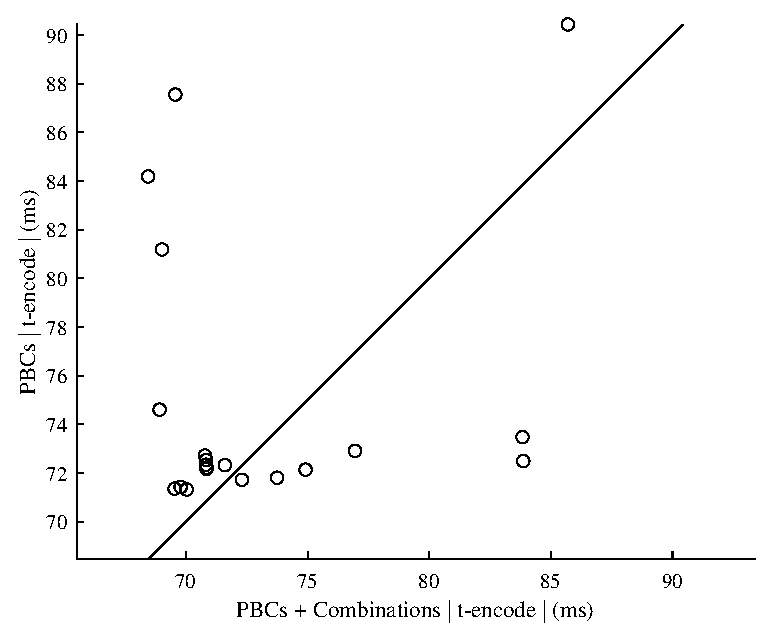
\includegraphics[height = 90mm]{Figures/opt_encode_2_1.eps}
    \captionsetup{justification=centering,margin=0cm}
    \caption{Average encoding time comparison, PBCs vs. PBCs + Combinations,\\ using Adder Networks}
    \label{opt_encode_2_1}
\end{figure}

\begin{figure}
    \centering
    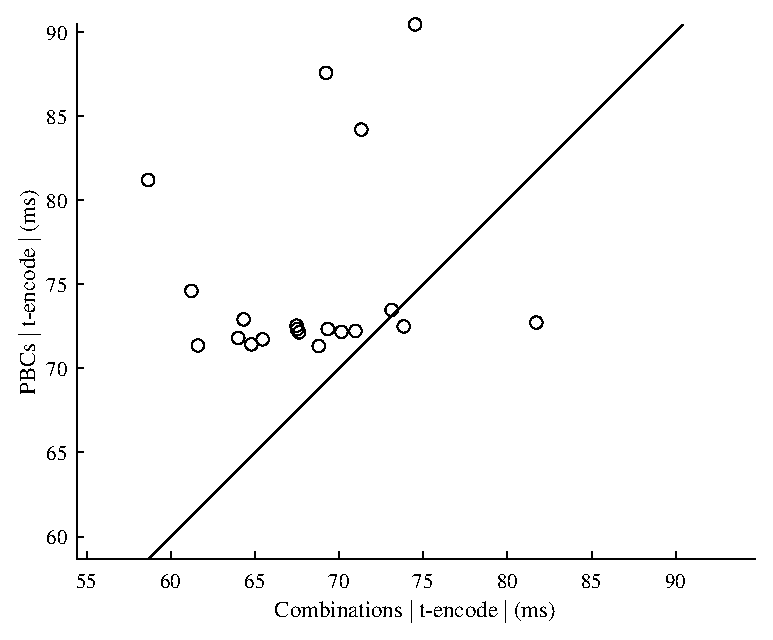
\includegraphics[height = 90mm]{Figures/opt_encode_3_1.eps}
    \captionsetup{justification=centering,margin=0cm}
    \caption{Average encoding time comparison, PBCs vs. Combinations,\\ using Adder Networks}
    \label{opt_encode_3_1}
\end{figure}

\begin{figure}
    \centering
    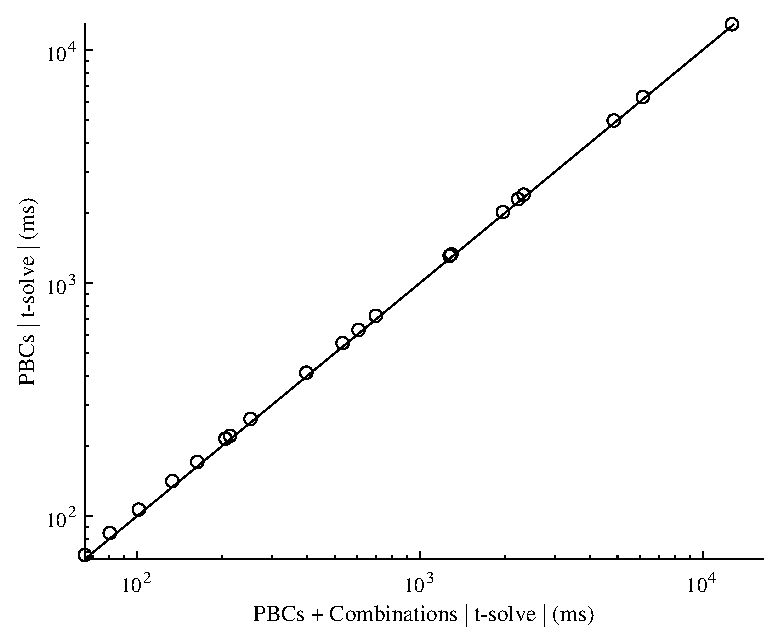
\includegraphics[height = 90mm]{Figures/opt_solve_2_1.eps}
    \captionsetup{justification=centering,margin=0cm}
    \caption{Average solving time comparison, PBCs vs. PBCs + Combinations,\\ using Adder Networks}
    \label{opt_solve_2_1}
\end{figure}

\begin{figure}
    \centering
    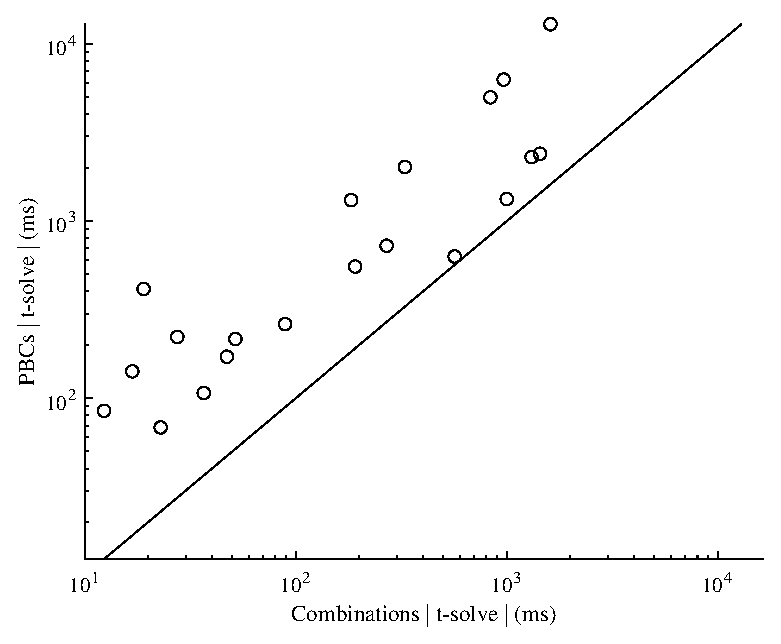
\includegraphics[height = 90mm]{Figures/opt_solve_3_1.eps}
    \captionsetup{justification=centering,margin=0cm}
    \caption{Average solving time comparison, PBCs vs. Combinations,\\ using Adder Networks}
    \label{opt_solve_3_1}
\end{figure}
}
\FloatBarrier

\begin{table}[t]
    \centering
    \renewcommand{\arraystretch}{1.5}
    \resizebox{\textwidth}{!}{
    \begin{tabular}{ |l|r|r|r|r|r|r|r|r|}
    \hline
    \multicolumn{1}{|c|}{\multirow{3}{*}{Variant}} & \multicolumn{3}{c|}{\makecell[c]{$t$-avg.\\(ms)}} & \multicolumn{3}{c|}{\makecell[c]{$t$-std.\\(ms)}} & \multicolumn{1}{c|}{\multirow{3}{*}{\#clauses}} & \multicolumn{1}{c|}{\multirow{3}{*}{\#variables}}\\\cline{2-7}
    & \multicolumn{1}{c|}{\multirow{2}{*}{encode}} & \multicolumn{2}{c|}{\makecell[c]{solve}} & \multicolumn{1}{c|}{\multirow{2}{*}{encode}} & \multicolumn{2}{c|}{\makecell[c]{solve}} &&\\\cline{3-4}\cline{6-7}
    && \makecell[c]{Sat4j} & \makecell[c]{MiniSat} & & \makecell[c]{Sat4j} & \makecell[c]{MiniSat} &&\\
    \hline
    9 Marks The Spot        &4428.02       & 170.90       &     1179.53      &211.03        & 36.76        &        519.18    & 727636 & 5994\\
    \hline
    Chess Sudoku            & 29.05       & 3.23        &      1061.05     &       1.10   &       0.43   &       241.94     &  8912 & 729\\
    \hline
    Fawlty Towers           & 65.38      &     11.10    &         904.62   &   12.31      &    0.71     &         127.42   & 17632& 2186 \\
    \hline
    Frozen Picnic           & 168.32      &    14.92    &         886.33   &    3.99      &      0.81    &         51.47   & 40519 & 5387\\
    \hline
    Mark 1                  &  28.60       &   8.18       &     903.05       &    2.12     &    0.50      &        52.05     &8839 & 729\\
        \hline
    Nurikabe Sudoku         & 77406.68      &        4145268.40       &          413259.82          &        3341.18       &        536495.31       &          5633.74         & 13904145 & 1169013\\
    \hline
    Sudoku Man Of Mystery   & 23.18        &     1.97     &      876.67      &   0.93       &  0.71        &         6.85     &  7399 & 729\\
    \hline
    The Miracle Thermo      & 739.77       &    446.32    &        1671.62   &    261.78   &     24.74    &        112.12    & 138743 & 5265\\
    \hline
    The Original Sandwich   &   1677.18    &    15408.00  &       2059.25    &    26.28    &   384.06    &       12.22     & 302640 & 42635\\
    \hline
    The Pyramid             &    48.68     &    219.07    &         1434.53  &    2.23      &    3.46    &         3.36     &15233& 1679\\
    \hline
    Thermo 2020             &  24.23       &     1.97    &         1355.67  &   1.09       &      0.66   &       54.23      & 7659 & 729\\
    \hline
    Thermo Couples          &  27.98       &    3.80      &          1354.52 &     0.85   &     0.55     &        8.19      & 8884 & 729\\
    \hline
    Thermo Squares          & 23.92        &    17.95     &        1362.25   &    0.74      &      0.67    &          54.87   & 7692 & 729\\
    \hline
    The Road To Genius      &   22.95       &    1.97      &      1364.20     &    0.81    &     0.74     &          56.83   &  7401 & 729\\
    \hline
    \end{tabular}
    }
    \renewcommand{\arraystretch}{1}
    
    \captionsetup{justification=centering,margin=2cm}
    \caption{CTCGH Sudokus, solving with Sat4j and MiniSat, \\PBC-Encoding with Adder Networks}
    
    \label{Experimnet:CTCGH}
\end{table}



\begin{table}[t]
    \renewcommand{\arraystretch}{1.5}
    \centering
    \resizebox{0.6\textwidth}{!}{
    
    \begin{tabularx}{30.56em}{|l|c|c|c|c|c|c|c|c|c|}
    \hline
    \multicolumn{1}{|c|}{\multirow{1}{*}{
     \belowbaseline[0ex]{~~~\rotatebox{45}{\parbox{3cm}{\raggedright{~Instance $\vert$ Rule}}}}}} &
     \belowbaseline[0ex]{\rotatebox{90}{\parbox{2.8cm}{\raggedright{~Normal Sudoku}}}} &
     \belowbaseline[0ex]{\rotatebox{90}{\parbox{2.8cm}{\raggedright{~Anti-Knight}}}} &
     \belowbaseline[0ex]{\rotatebox{90}{\parbox{2.8cm}{\raggedright{~Killer Sudoku}}}} &
     \belowbaseline[0ex]{\rotatebox{90}{\parbox{2.8cm}{\raggedright{~Arrowheads}}}} &
     \belowbaseline[0ex]{\rotatebox{90}{\parbox{2.8cm}{\raggedright{~Thermometers}}}} &
     \belowbaseline[0ex]{\rotatebox{90}{\parbox{2.8cm}{\raggedright{~Sandwich Sum}}}} &
     \belowbaseline[0ex]{\rotatebox{90}{\parbox{2.8cm}{\raggedright{~Secret Direction}}}} &
     \belowbaseline[0ex]{\rotatebox{90}{\parbox{2.8cm}{\raggedright{~Fawlty Towers}}}} &
     \belowbaseline[0ex]{\rotatebox{90}{\parbox{2.8cm}{\raggedright{~Nurikabe Sudoku}}}}\\
    \hline 
    9 Marks The Spot & $\times$& & & & & & $\times$& & \\
    \hline 
    Chess Sudoku &$\times$ & $\times$& & & $\times$& & & & \\ 
    \hline 
    Fawlty Towers &$\times$ & & & & & & &$\times$ & \\
    \hline 
    Frozen Picnic &$\times$ & & &$\times$ &$\times$ &$\times$ & & & \\
    \hline 
    Mark 1 &$\times$ &$\times$ & & & $\times$& & & & \\
    \hline 
    Nurikabe Sudoku & $\times$& & & & & & & & $\times$\\
    \hline 
    Sudoku Man Of Mystery & $\times$& & & & & & & & \\
    \hline 
    The Miracle Thermo &$\times$ & & & &$\times$ & & & & \\
    \hline 
    The Original Sandwich & $\times$& & & & &$\times$ & & & \\
    \hline 
    The Pyramid &$\times$ &$\times$ & $\times$& & & & & & \\
    \hline 
    Thermo 2020 & $\times$& & & &$\times$ & & & & \\
    \hline 
    Thermo Couples & $\times$&$\times$ & & &$\times$ & & & & \\
    \hline 
    Thermo Squares &$\times$ & & & & $\times$& & & & \\ 
    \hline 
    The Road To Genius &$\times$ & & & & & & & & \\ 
    \hline
    \end{tabularx}
    }
    \renewcommand{\arraystretch}{1}
    \caption{Sudoku Puzzle instances and their rules.}
    \label{tab:InstanceRule}
\end{table}

